\documentclass{article}

\usepackage[utf8]{inputenc}
\usepackage[brazil]{babel}

\title{Exercício 6: Adaline}
\author{Rúbia Reis Guerra \\ 2013031143}

\usepackage{Sweave}
\begin{document}
\Sconcordance{concordance:adaline.tex:adaline.Rnw:%
1 8 1 1 0 21 1 1 2 1 0 3 1 1 2 1 0 5 1 3 0 1 2 1 1 1 4 3 0 2 1 1 3 1 0 %
1 3 1 0 2 1 1 3 1 0 2 1 1 3 1 0 1 1 1 3 1 0 1 3 4 0 1 2 1 1 1 4 3 0 1 1 %
1 3 2 0 1 1 1 2 1 0 1 1 1 4 3 0 1 2 5 0 1 2 1 5 4 0 1 1 1 2 1 0 1 1 1 4 %
3 0 1 2 5 0 1 2 2 1 1 3 7 0 1 3 7 0 1 2 12 1 1 2 1 0 3 1 1 2 1 0 5 1 3 %
0 1 2 1 1 1 4 3 0 2 1 1 3 1 0 1 3 1 0 2 1 1 3 1 0 2 1 1 3 1 0 2 1 1 3 1 %
0 1 3 4 0 1 2 1 1 1 3 2 0 1 7 6 0 1 1 1 3 6 0 1 2 1 4 3 0 1 1 1 3 6 0 1 %
2 1 4 3 0 1 1 1 2 1 0 1 1 1 3 2 0 1 2 5 0 1 2 2 1 1 4 8 0 1 2 7 0 1 2 1 %
1}

\maketitle

\section{Adaline}
A atividade proposta teve como objetivo o estudo e a implementação de um rede neural artificial de camada única Adaline A diferença entre Adaline e o perceptron padrão (McCulloch-Pitts) é que na fase de aprendizagem, os pesos são ajustados de acordo com a soma ponderada das entradas (a rede). No perceptron padrão, a rede é passada para a função de ativação (transferência) e a saída da função é usada para ajustar os pesos.

\section{Funções \textit{yadaline} e \textit{trainadaline}}
Para esta atividade, foi proposta a implementação das funções \textit{yadaline}, correspondente à função de custo do Adaline, e \textit{trainadaline}, que calcula e ajusta o vetor de pesos por correção de erros, descritas nas notas de aula disponibilizadas.

\section{Exercício 1}

\subsection{Parâmetros}
Os parâmetros foram definidos em:
\begin{itemize}
\item Passo de atualização de $w$ (eta): 0.1
\item Tolerância (tol): 0.01
\item Número máximo de épocas (maxepocas): 10000
\item Adição de bias a x (par): TRUE
\item Porcentagem do conjunto de dados para treino (ptrain): 70\%
\item Porcentagem do conjunto de dados para teste (ptest): 30\%
\end{itemize}
\begin{Schunk}
\begin{Sinput}
> rm(list=ls())
> library('plot3D')
> source('yadaline.R')
> source('trainadaline.R')
> # Parâmetros #
> eta <- 0.1
> tol <- 0.01
> maxepocas <- 10000
> par <- 1
> ptrain <- 0.7
> ptest <- 1 - ptrain
\end{Sinput}
\end{Schunk}

\subsection{Treinamento e Teste}
\begin{Schunk}
\begin{Sinput}
> ##########################################
> # Exercício 1 #
> ex1_x <- as.matrix(read.table('Ex1_x'))
> ex1_y <- as.matrix(read.table('Ex1_y'))
> ex1_t <- as.matrix(read.table('Ex1_t'))
> # Amostragem: treino e teste #
> index <- sample(2, nrow(ex1_x), replace=TRUE, prob=c(ptrain,ptest))
> # Treino #
> xtrain <- as.matrix(ex1_x[which(index==1),])
> ytrain <- as.matrix(ex1_y[which(index==1)])
> ttrain <- as.matrix(ex1_t[which(index==1)])
> # Teste #
> xtest <- as.matrix(ex1_x[which(index==2),])
> ytest <- as.matrix(ex1_y[which(index==2)])
> ttest <- as.matrix(ex1_t[which(index==2)])
> # Treinamento #
> train <- trainadaline(xtrain, ytrain, eta, tol, maxepocas, par)
> wt <- train$wt
> # Teste #
> test <- yadaline(xtest, wt, par)
> # MSE #
> mse <- sum((ytest - test)^2)/(length(ytest))
\end{Sinput}
\end{Schunk}

\subsection{Plot: Treinamento e Teste}
\begin{Schunk}
\begin{Sinput}
> # Plot: treinamento #
> plot(ex1_t,ex1_x,type='o',xlim=c(min(ex1_t),max(ex1_t)), 
+      ylim=c(min(ex1_x),max(ex1_x)),xlab='t',ylab='',col='red')
> par(new=T)
> plot(ttrain, xtrain, type='p', pch=19, col='red',
+      xlim=c(min(ex1_t),max(ex1_t)), 
+      ylim=c(min(ex1_x), max(ex1_x)), ylab = '',xlab='')
> par(new=T)
> plot(ex1_t,ex1_y,type='o',xlim=c(min(ex1_t),max(ex1_t)),
+      ylim=c(min(ex1_x),max(ex1_x)),ylab='',xlab='',col='blue')
> par(new=T)
> plot(ttrain, ytrain, type='p', pch=19, col='blue',
+      xlim=c(min(ex1_t),max(ex1_t)), 
+      ylim=c(min(ex1_x), max(ex1_x)), ylab = '',xlab='',
+      sub="Amostras preenchidas foram usadas para treinamento")
> legend(0.2, -0.4, legend=c("Entrada", "Saída Original"),
+        col=c("red", "blue"), lty=1:2, cex=0.8)
\end{Sinput}
\end{Schunk}
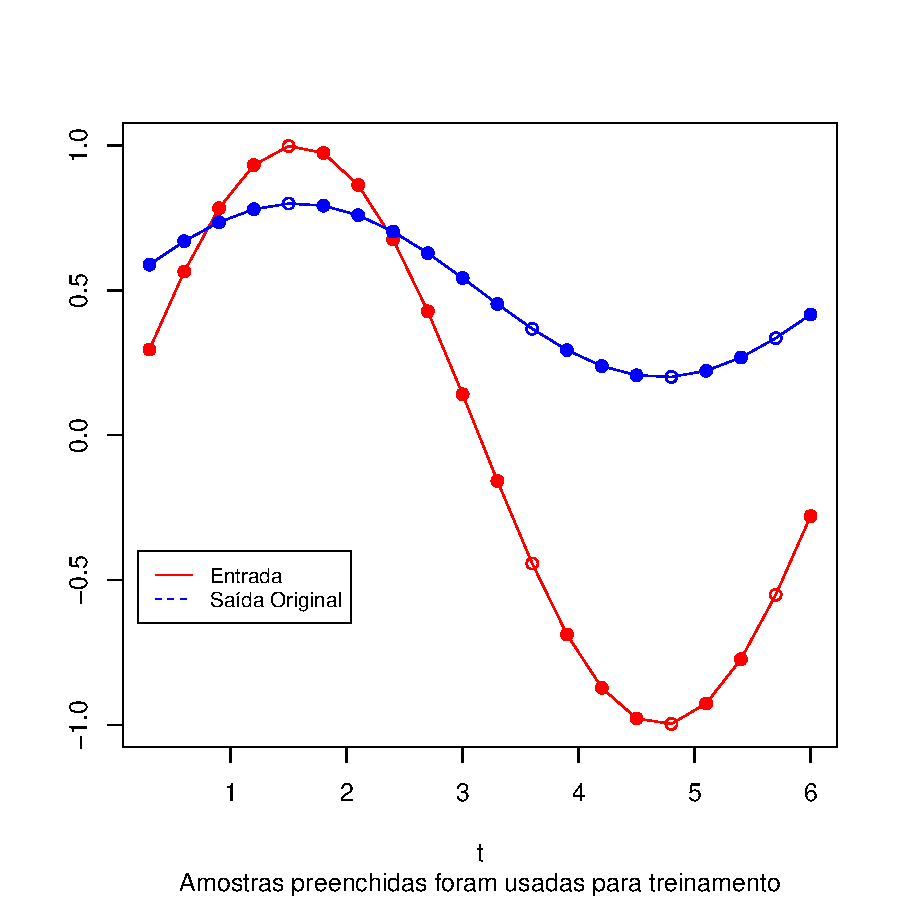
\includegraphics{adaline-003}

\begin{Schunk}
\begin{Sinput}
> # Plot: Teste #
> plot(ex1_t,ex1_x*wt[2]+wt[1],type='o',
+      xlim=c(min(ex1_t),max(ex1_t)),
+      ylim=c(min(ex1_x),max(ex1_x)),ylab='',xlab='',col='blue')
> par(new=T)
> plot(ex1_t,ex1_y,type='o',xlim=c(min(ex1_t),max(ex1_t)),
+      ylim=c(min(ex1_x),max(ex1_x)),ylab='',col='green',xlab='')
> par(new=T)
> plot(ttest, ytest, type='p', pch=19, col='green',
+      xlim=c(min(ex1_t),max(ex1_t)), 
+      ylim=c(min(ex1_x), max(ex1_x)), ylab = '',xlab='',
+      sub="Amostras preenchidas foram usadas para teste")
> legend(0.2, -0.4, legend=c("Saída Prevista", "Saída Original"),
+        col=c("blue", "green"), lty=1:3, cex=0.8)
\end{Sinput}
\end{Schunk}
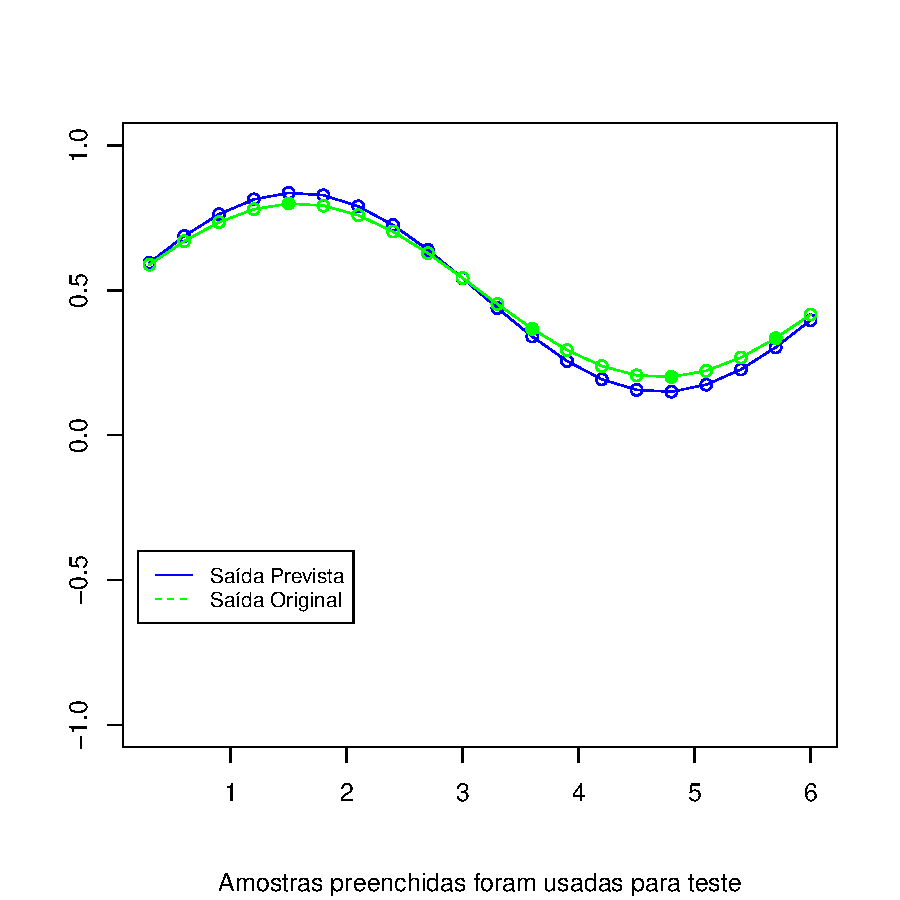
\includegraphics{adaline-004}

\subsection{Resultados}
Foram obtidos os seguintes parâmetros (a, b) e erro médio quadrático:
\begin{Schunk}
\begin{Sinput}
> # Parâmetros do modelo#
> sprintf("a = %1$.3f, b = %2$.3f", wt[2], wt[1])
\end{Sinput}
\begin{Soutput}
[1] "a = 0.344, b = 0.493"
\end{Soutput}
\begin{Sinput}
> # MSE #
> sprintf("MSE = %.3f%%", 100*mse)
\end{Sinput}
\begin{Soutput}
[1] "MSE = 0.143%"
\end{Soutput}
\end{Schunk}

\section{Exercício 2}

\subsection{Parâmetros}
Os parâmetros foram definidos em:
\begin{itemize}
\item Passo de atualização de $w$ (eta): 0.1
\item Tolerância (tol): 0.01
\item Número máximo de épocas (maxepocas): 10000
\item Adição de bias a x (par): TRUE
\item Porcentagem do conjunto de dados para treino (ptrain): 70\%
\item Porcentagem do conjunto de dados para teste (ptest): 30\%
\end{itemize}
\begin{Schunk}
\begin{Sinput}
> rm(list=ls())
> library('plot3D')
> source('yadaline.R')
> source('trainadaline.R')
> # Parâmetros #
> eta <- 0.1
> tol <- 0.01
> maxepocas <- 10000
> par <- 1
> ptrain <- 0.7
> ptest <- 1 - ptrain
\end{Sinput}
\end{Schunk}

\subsection{Treinamento e Teste}
\begin{Schunk}
\begin{Sinput}
> ##########################################
> # Exercício 2 #
> x <- as.matrix(read.table('x'))
> y <- as.matrix(read.table('y'))
> t <- as.matrix(read.table('t'))
> # Amostragem: treino e teste #
> index <- sample(2, nrow(x), replace=TRUE, prob=c(ptrain,ptest))
> # Treino #
> xtrain <- as.matrix(x[which(index==1),])
> ytrain <- as.matrix(y[which(index==1)])
> ttrain <- as.matrix(t[which(index==1)])
> # Teste #
> xtest <- as.matrix(x[which(index==2),])
> ytest <- as.matrix(y[which(index==2)])
> ttest <- as.matrix(t[which(index==2)])
> # Treinamento #
> wt <- c()
> train <- trainadaline(xtrain, ytrain, eta, tol, maxepocas, par)
> wt <- train$wt
> # Teste #
> test <- yadaline(xtest, wt, par)
> # MSE #
> mse <- sum((ytest - test)^2)/(length(ytest))
\end{Sinput}
\end{Schunk}

\subsection{Plot: Treinamento e Teste}
\begin{Schunk}
\begin{Sinput}
> # Plot #
> cores <- rainbow(dim(x)[2])
> for(i in 1:(dim(x)[2]-1))
+ {
+   plot(t,x[,i],type='o',pch=21, ylab='x',xlim=c(0.1*pi,2*pi),
+        col=cores[i],  ylim=c(min(x),max(x)),
+        sub="Sinais de entrada")
+   par(new=T)
+ }
> i <- i + 1
> plot(t,x[,i],type='o',pch=21, ylab='x',xlim=c(0.1*pi,2*pi),
+        col=cores[i],  ylim=c(min(x),max(x)),
+        sub="Sinais de entrada")
\end{Sinput}
\end{Schunk}
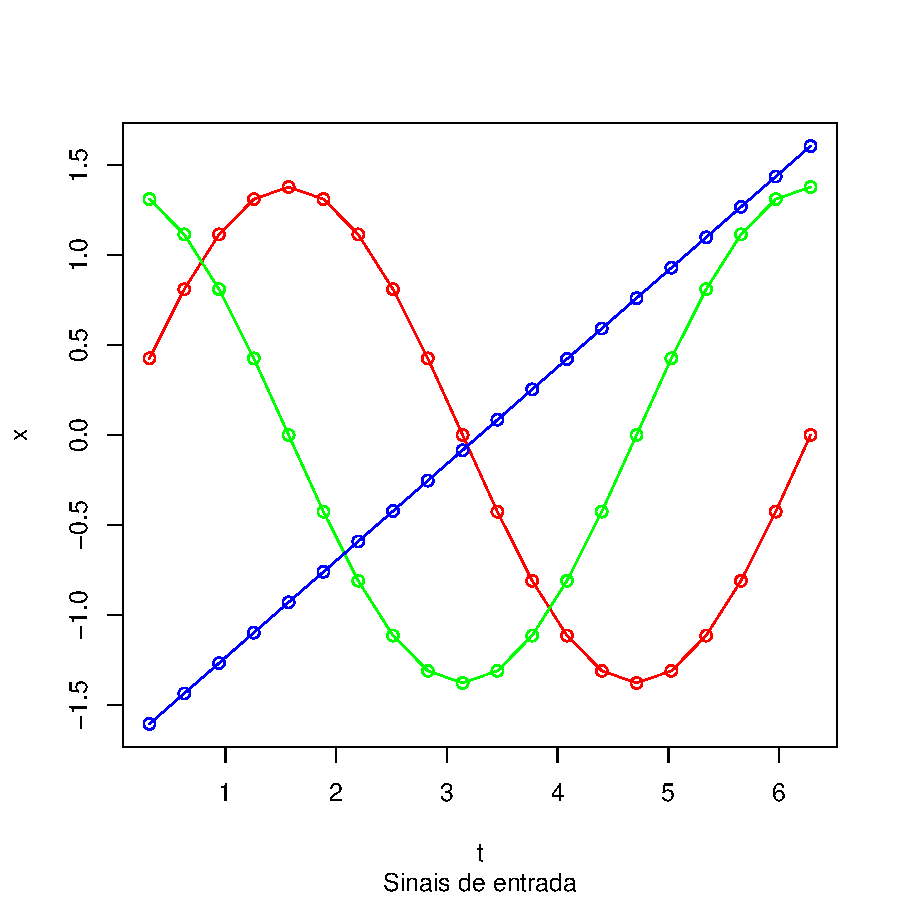
\includegraphics{adaline-008}

\begin{Schunk}
\begin{Sinput}
> plot(t,y,type='o', col='orange', 
+      xlim=c(min(t),max(t)), 
+      ylim=c(min(y), max(y)), ylab='y',xlab='t')
> par(new=T)
> plot(ttrain, ytrain, type='p', pch=19, col='orange',
+      xlim=c(min(t),max(t)), 
+      ylim=c(min(y), max(y)), ylab = '',xlab='',sub="Saída original")
\end{Sinput}
\end{Schunk}
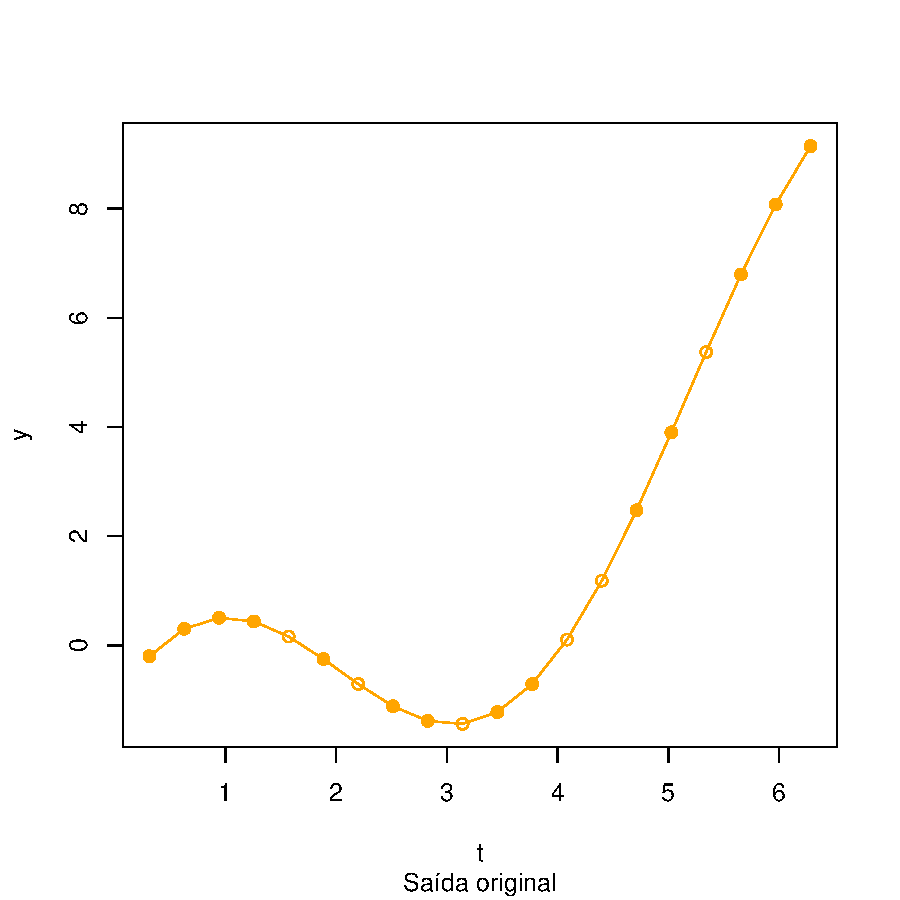
\includegraphics{adaline-009}

\begin{Schunk}
\begin{Sinput}
> plot(t,(x[,1]*wt[2]+x[,2]*wt[3]+x[,3]*wt[4]+wt[1]),
+      type='o',xlim=c(0.1*pi,2*pi),
+      ylim=c(min(y),max(y)),ylab='',col='black')
> par(new=T)
> plot(t,y,type='o', col='orange', xlim=c(min(t),max(t)), 
+      ylim=c(min(y), max(y)), ylab='y',xlab='t')
> par(new=T)
> plot(ttest, ytest, type='p', pch=19, col='orange',
+      xlim=c(min(t),max(t)), ylim=c(min(y), max(y)), 
+      ylab = '',xlab='',sub="Saída prevista")
> legend(0.2, 8, legend=c("Original", "Previsto"),
+        col=c("orange", "black"), lty=1:2, cex=0.8)
\end{Sinput}
\end{Schunk}
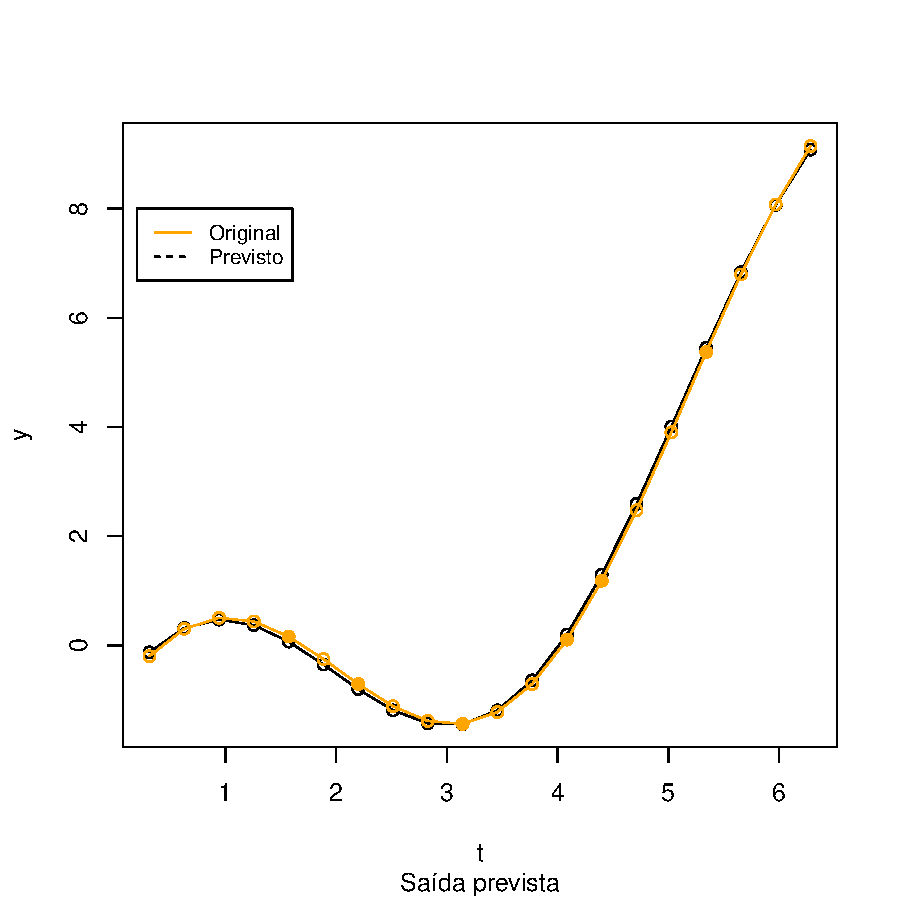
\includegraphics{adaline-010}

\subsection{Resultados}
Foram obtidos os seguintes parâmetros (a, b, c, d) e erro médio quadrático:
\begin{Schunk}
\begin{Sinput}
> # Parâmetros do modelo #
> sprintf("a = %1$.3f, b = %2$.3f, c = %3$.3f, d = %4$.3f", 
+         wt[1], wt[2], wt[3], wt[4])
\end{Sinput}
\begin{Soutput}
[1] "a = 1.578, b = 0.888, c = 2.014, d = 2.942"
\end{Soutput}
\begin{Sinput}
> # MSE #
> sprintf("MSE = %.3f%%", 100*mse)
\end{Sinput}
\begin{Soutput}
[1] "MSE = 0.767%"
\end{Soutput}
\end{Schunk}

\end{document}
